\documentclass[fleqn,10pt]{wlscirep}

\usepackage{graphicx}
\usepackage{grffile}
\usepackage{textcomp}

\newcommand{\secref}[1]{Section~\ref{sec:#1}}
\newcommand{\tabref}[1]{Table~\ref{tab:#1}}
\newcommand{\figref}[1]{Figure~\ref{fig:#1}}

\newcommand{\beginsupplement}{%
        \setcounter{table}{0}
        \renewcommand{\thetable}{S\arabic{table}}%
        \setcounter{figure}{0}
        \renewcommand{\thefigure}{S\arabic{figure}}%
     }

\newcommand{\textapprox}{\raisebox{0.5ex}{\texttildelow}}

\graphicspath{{./images/}}


\title{Non-Parametric Mixture Modeling for Pediatric Precision Oncology}

\author[1,*]{Jacob Pfeil}
\author[1]{Geoff Lyle}
\author[1]{Lauren Sanders}
\author[1]{Katrina Learned}
\author[1]{Ellen Kephart}
\author[1]{Ann Durbin}
\author[1]{Holly Beale}
\author[1]{Olena Morozova}
\author[1]{Sofie Salama}
\author[1]{David Haussler}
\affil[1]{University of California, Santa Cruz, Biomolecular Engineering, Santa Cruz, 95064, United States}

\affil[*]{jpfeil@ucsc.edu}

%\keywords{Keyword1, Keyword2, Keyword3}

% TODO
% Write results 
% - make figure showing a normally distributed gene expression distribution
% - make neuroblastoma MYCN distribution
% Write methods 
% Write discussion
% Write introduction

\begin{abstract}
Precision oncology is changing the way medicine is practiced by incorporating high-throughput genomic analyses and data analytics. The field has focused on genomic variants, but gene expression data is becoming an additional tool for clinicians to improve patient outcomes. Here, we discuss a novel computational approach for identifying gene expression subtypes that may be helpful for future drug development and risk stratification. We apply this approach to synthetic data as well as patient data from the Cancer Genome Atlas Project. \end{abstract}
\begin{document}

\flushbottom
\maketitle
% * <john.hammersley@gmail.com> 2015-02-09T12:07:31.197Z:
%
%  Click the title above to edit the author information and abstract
%
\thispagestyle{empty}


\section*{Introduction}

% The Introduction section, of referenced text\cite{Figueredo:2009dg} expands on the background of the work (some overlap with the Abstract is acceptable). The introduction should not include subheadings.
% Overview of field? I really don't want to start with the whole DNA sequencing has become so popular. Let's write an outline first.
Cancer gene expression analysis has traditionally been used to compare the expression between two groups. The heterogeneity of tumor populations warrants an analysis that can identify differences across multiple subtypes with overlapping features. Differentiating expression at this level has been a challenge, so single-sample approaches have become more popular. However, the single-sample approach does not identify structure within a disease population that would improve the analysis of individual patients. 

% TCGA Gene Expression Data

Many researchers have proposed a mixture modeling approach for differential expression analysis, but a mixture modeling approach has not been adopted by the gene expression analysis community (TODO: ADD REFERENCES TO GENE EXPRESSION MIXTURE MODEL PAPERS). One reason for this is the lack of tools to facilitate this type of analysis. These models are difficult to implement and pre-implemented tools are not well designed for cancer gene expression analysis. There has also been an insufficient number of tissue-specific gene expression profiles to differentiate molecular subtypes. However, the work of TCGA, TARGET, and public repositories not make more sophisticated gene expression analyses possible. 

Most genes' expression distribution is approximately normally distributed once normalized using a log transformation \cite{zwiener2014transforming}. 

% Other approaches in the field
% Here I'll talke about the gene set enrichment approaches

% Overview of method
Commonly used gene expression analyses are used to compare two populations or single samples, but methods are needed to find subtypes within a disease population. Supervised learning approaches like linear regression use known categorical information to learn differences between groups, but these methods are not able to detect subtle differences across a disease population without knowing the differences beforehand. Unsupervised methods are needed to subtype diseases, but one of the limitations in an unsupervised approach is that it is often necessary to specify the number of expected groups beforehand, which limits the ability to discover novel subtypes.

The goal of the hydra algorithm is to enrich for genes of interest by removing genes that are unimodally expressed across a disease cohort. Biomarker development requires gene expression distributions that are detectable in noisy gene expression data. Thus, potential biomarkers must be multimodally expressed and we can use this assumption to identify biomarkers for subtyping tumors and identifying novel drug targets. Multimodally expressed genes may be useful for subtyping tumors, but often there is a variable of interest that covaries with an expression distribution. Once the feature space has been reduced to a smaller size, then the analysis become powered to detected coordinated expression by identifying multivariate clusters. This allows the researchers to investigate the correlation of several genes associated with a variable of interest which will lead to robust detection of expression subtypes and robust gene expression signatures.

Hydra is built upon the Bayesian non-parametric python toolbox bnpy \cite{hughes2014bnpy}. The benefit of a non-parametric approach is that the number of clusters does not need to specified because the algorithm is able to infer the number of clusters from the data. The bnpy library provides a flexible set of tools for performing Dirichlet process mixture modeling. Here, we use the Dirichlet process mixture modeling functions to identify multimodally expressed genes in the univariate setting and a bivariate setting if a covariate variable is provided. The bnpy implementation is fast and can scale to tens of thousands of genes.

The input for the hydra approach is a genes by samples matrix. The Dirichlet process mixture model has the property that as the number of samples increases, the number of clusters identified also increases. The first pass of the hydra pipeline is to identify all of the genes that are multimodally expressed and thus a potential biomarker. If a covariate is provided, then the hydra method does a bivariate clustering to identify genes that are differentially expressed and statistically different in the covariate dimension using a Kruskal-Wallis test \cite{mckight2010kruskal}. The goal of this analysis is to identify the genes that have a strong signal and may subtype tumors. The multimodally expressed genes are then assembled into a multivariate mixture modeling analyis to find coordinated expression of genes that subtype tumors. We have found that these expression networks show related biological function and can be used to identify pathway-level expression for subtyping tumors.

%%%%%%%%%%%%%%%%%%%%%%%%%%%%%%%%%%
% Figure describing hydra %
%%%%%%%%%%%%%%%%%%%%%%%%%%%%%%%%%%
\begin{figure}
	\centering
	\includegraphics[width=0.5\linewidth]{images/hydra-overview@2x.png}
	\caption{Hydra Method Overview}
	\label{sfig:hydra-overview}
\end{figure}

\section*{Results}

\subsection*{Synthetic Data Analysis}
Synthetic data was generated to assess the performance of the hydra mixture modeling approach. The synthetic data was generated from GTEx normal muscle tissue and randomly assigning a subset of samples to have higher expression for a subset of the MSigDB hallmark genes. We compare our method with single sample gene set enrichment analysis \cite{barbie2009systematic} and gene set variation analysis \cite{hanzelmann2013gsva}. The hydra method performed best across the 34 Hallmark gene sets. We also compare the area under the curve from the receiver operator characteristics plot to the mean expression across the Hallmark gene sets and noticed that the ranking methods have lower predictive performance when the background expression for the gene set increases.

For instance, we compare the performance across these methods for the Hallmark Glycolysis gene set and the Hallmark Oxidative Phosphorylation gene set. The Hallmark Glycoloysis gene set has lower background expression than the Hallmark Oxidative Phosphorylation gene set (TODO: Add mean expression). We found that the ssGSEA method performed comparatively to the hydra method when the background expression is lower, but when the background expression is higher, the ssGSEA method's performance wanes and this effect is related to the effect size. A larger effect size for the change in expression decreases the effect of the background expression.

Across the 34 Hallmark gene sets with at least 100 genes, the hydra approach had a mean AUC of 

%%%%%%%%%%%%%%%
% ROC Plot Figure %
%%%%%%%%%%%%%%%

\begin{figure}
	\centering
	\includegraphics[width=0.75\linewidth]{images/figure-2-roc-curves@2x.png}
	\caption{ROC Plot Curves for Assessing the Performance of Pathway Enrichment Tools.}
	\label{sfig:rocplot}
\end{figure}

 


TODO: Need to compare the small effect size and the large effect size 

\subsection{Cell Line Validation}
\begin{figure}
	\centering
	\includegraphics[width=0.75\linewidth]{images/rough-cell-line-validation.png}
	\caption{Cell Line Validation}
	\label{sfig:cellline}
\end{figure}

\subsection*{Immune Subtype Validation}
Whether pediatric cancer in general has a significant immune component is an active area or research. The success of checkpoint therapies in adult cancers has not been as strongly adopted in pediatric cancers because these therapies tend to do better in patients with a high mutation burden. Pediatric cancers generally have low mutation burdens. However, several groups have found elevated checkpoint marker expression in pediatric cancers \cite{majzner2017assessment,saletta2017programmed,nowicki2016prospective}, which suggests that immunosuppressive mechanisms are active in pediatric cancers and may need further characterization to identify therapeutic opportunities. 

We show that the hydra approach is able to subtype patients using immune gene sets in a way that correlates with the computational staining of haemotoxylin and eosin (H\&E) staining. We analyzed the TCGA skin cutaneous melanoma data set (TODO: N=X)

\subsection*{Neuroblastoma Transposable Element Analysis}
One theory for way ATRX deleted samples have higher immune marker infiltrate is that dysregulation of ATRX function leads to increased expression of transposable elements which induces a DAMP response. Transposable elements have been shown to induce innate and adaptive immune responses, so the nature of the transposable elements may play a role in the type of immune response the occurs. The transposable element sequences may lead to the generation of antigens that can be used for treatment of neuroblastoma. 

In order to investigate the transposable element expression in neuroblastoma, we applied two state-of-the-art methods. The first is the salmonTE algorithm and the second is the BLANK algorithm. We used two background cohorts to quantify transposable element expression. The first is tissue matched patients that were identified as having significantly lower expression of immune markers. The second is the UVM TCGA cohort which has been used in other studies as a negative control for immune active tumors \cite{bindea2013spatiotemporal,thorsson2018immune}.


\section*{Discussion}

The Discussion should be succinct and must not contain subheadings.

One of the benefits of this approach is that this provides a framework for understanding a population of patients and can identify subtypes that may benefit from future drug development. Investigation into subtype specific expression may also identify opportunities to repurpose available therapies for other diseases. This is particularly useful for pediatric cancer gene expression analysis where drug development has lagged and there is a need for novel therapies. 

One of the limitations of a non-parametric ranking approach to gene set enrichment is that it cannot account for the dynamic range in expression for a gene in a single-sample context. Therefore, we hypothesized that a GSEA method approach that does not account for this information will suffer if the background expression for a gene set is high. We see this in the HALLMARK Oxidative Phosphorylation analysis where the ssGSEA suffers from poor performance because the background expression is higher and thus is not well suited to identify subtle changes in expression.


\section*{Methods}

%Topical subheadings are allowed. Authors must ensure that their Methods section includes adequate experimental and characterization data necessary for others in the field to reproduce their work.

\subsection{Synthetic Data Generation}
The MSigDB Hallmark gene sets were used to simulate biological pathway expression that reflects the gene set properties of a typical gene expression analysis \cite{liberzon2015molecular,liberzon2011molecular}. We also needed a large cohort of human tissue samples to infer differentially expressed genes. We used the GTEx skeletal muscle cohort \cite{consortium2013genotype}. To simulate subtype specific expression, we randomly sampled 25\% of the patient population and then we sampled from a normal distribution centered at 0.5 with a standard deviation of 0.5. We then added this value to 25\% of the genes in each Hallmark gene set to simulate coordinated expression of genes within a biological gene set.

We compared the predictive performance for identifying enriched genes using healthy tissue samples collected as part of the Genotype-Tissue Expression (GTEx) project \cite{lonsdale2013genotype}. The Molecular Signatures Database (MSigDB) provides a large set of curated gene lists for identifying biological functions for precision medicine applications. We used the Hallmark MSigDB gene sets to select genes with related biological functions and correlated expression \cite{liberzon2015molecular}. We then randomly sampled GTEx skeletal muscle samples, modified their expression values for a subset of the gene set genes. We did this process twice to generate synthetic training and test data. The same genes were used in the test and training data, but the values were sampled independently from a normal distribution at varying mean differences. 

We applied this analysis to all of the Hallmark gene sets, but we are showing two illustrative examples here (TODO: add figure ref). The Hallmark Glycolysis gene set includes 199 genes involved in glycolysis and gluconeogenesis. We sample 25\% of these genes to be differentially expressed and sampled a difference in expression value from a normal $\mathcal{N}(0.5, 0.5)$ or a $\mathcal{N}(1, 0.5)$. If this difference caused a negative expression value, then we set the expression value to be zero. The GTEx expression TPM values were generated using the Toil RNA-Seq pipeline \cite{vivian2017toil}. The reciever operator curves (ROC) were generated for the hydra, ssGSEA, and GSVA methods. The hydra method performed the best with an AUC (area under the curve) of X, but the ssGSEA method was comparable with an AUC of blank. The GSVA method performed the worst with an AUC of BLANK.



\bibliography{reference}

\section*{Acknowledgements (not compulsory)}

Acknowledgements should be brief, and should not include thanks to anonymous referees and editors, or effusive comments. Grant or contribution numbers may be acknowledged.

\section*{Author contributions statement}

J.P. conceived the analysis, conducted the analysis, and wrote the paper. O.M., H.B., S.S., and D.H. reviewed the results and contributed feedback. All authors reviewed the manuscript. 

\section*{Additional information}

To include, in this order: \textbf{Accession codes} (where applicable); \textbf{Competing financial interests} (mandatory statement). 

The corresponding author is responsible for submitting a \href{http://www.nature.com/srep/policies/index.html#competing}{competing financial interests statement} on behalf of all authors of the paper. This statement must be included in the submitted article file.

\beginsupplement
\section*{Supplementary Information}

\subsection*{Cancer Gene Expression Distributions are Multi-Modal}
\subsubsection*{Modes Correspond to Sex-Specific Expression}
Genes are expressed at different levels for different tissues. In addition to tissue specific expression, there are also biological features that influence gene expression across individuals. For example, age and gender are correlated with expression of some genes. A varying effects model where the mean and the effect of biological features change depending on the tissue can be used to make better predictions of gene expression. For example, a hierarchical model can identify sex-linked expression, but the current pan-cancer and pan-disease analyses are not able to detect sex-linked expression. An example of sex-linked expression that has been associated with cancer is the XIST gene \cite{yildirim2013xist}. XIST controls X-chromosome silencing in females and is not usually expressed in males (\figref{xist}). This is a clear example where assuming male and female gene expression comes from the same distribution leads to an exaggerated estimation of the outlier threshold. It is therefore difficult to identify potential cases where under-expression of XIST in females may contribute to their cancer. While the incidence of cancer is equal across boys and girls, boys tend to respond worse to therapy. An investigation into sex-linked gene expression may yield insights into the differences in response to cancer therapies for boys and girls. 

%%%%%%%%%%%%%%%
% XIST Figure %
%%%%%%%%%%%%%%%

\begin{figure}
\centering
\includegraphics[width=0.75\linewidth]{images/xist-fig-2017-12-28.png}
\caption{Example of gender-specific expression that can be modeled in a hierarchical model. The XIST gene is involved in X chromosome silencing, so XIST is not expressed for males. XIST has been linked to cancer, but the Treehouse model overestimates the variance in XIST expression because females and males are modeled together. The proposed hierarchical model learns the differences between male and female XIST expression for improved model fit.}
\label{sfig:xist}
\end{figure}


%%%%%%%%%%%%%%%%%%%%%%%%%%
% MYCN Validation Figure %
%%%%%%%%%%%%%%%%%%%%%%%%%%

\begin{figure}
	\centering
	\includegraphics[width=0.75\linewidth]{images/MYCN-Figure.png}
	\caption{MYCN Validation}
	\label{sfig:mycn}
\end{figure}



\end{document}